\section{Introduction}
% no \IEEEPARstart
In early February 2012 the director of the Philadelphia Science Festival asked the Drexel Autonomous Systems Lab (DASL)\footnote{Drexel Autonomous Systems Lab: http://dasl.mem.drexel.edu}\label{foot:dasl} if they could have their adult-size humanoid robot Jaemi Hubo throw the ceremonial first pitch at the second annual \textit{Science Night at the Ballpark}.  On April 28th, 2012 Hubo successfully threw the first pitch at the Philadelphia Phillies Vs. Chicago Cubs game, see Fig.~\ref{fig:hubo-throw}.  This document describes, analyses and tests three different approaches to having an adult-size humanoid robot throw the first pitch.  

\begin{figure}[t]
  \centering
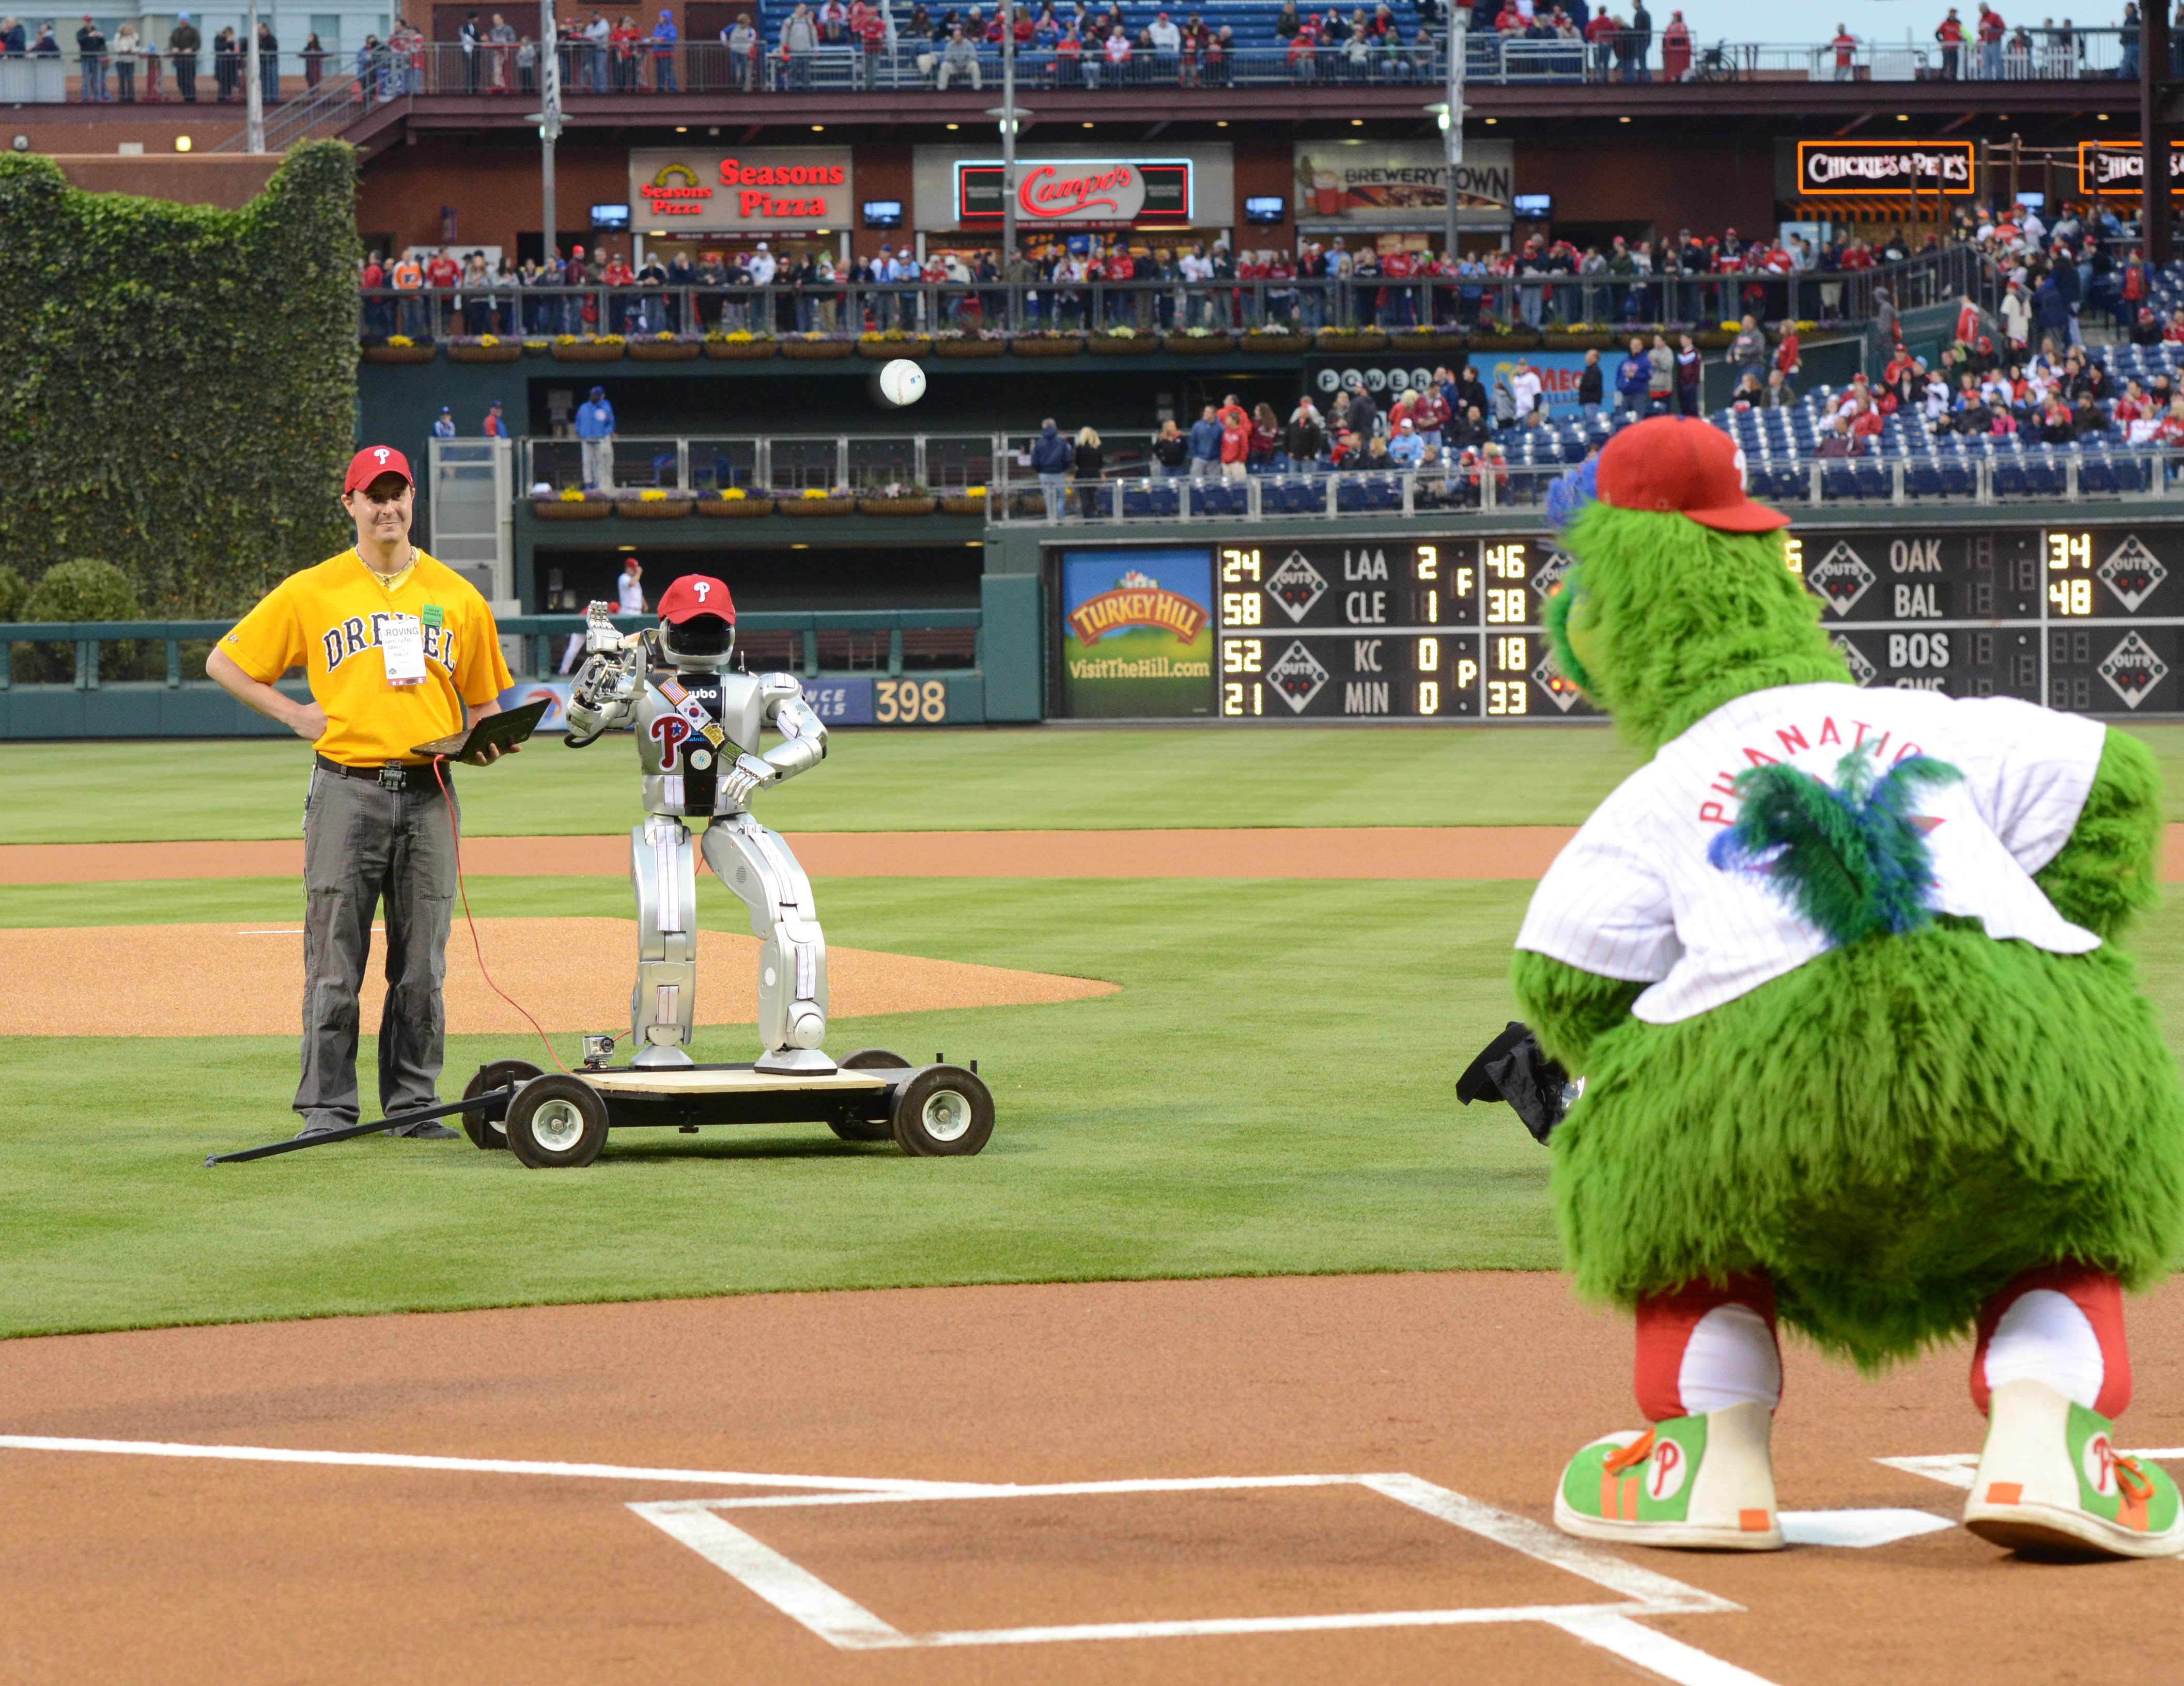
\includegraphics[width=1.0\columnwidth]{./pix/hubo-pitch.png}
  \caption{Hubo successfully throwing the first pitch at the second annual Philadelphia Science Festival event Science Night at the Ball Park on April 28th, 2012.  The game was between the Philadelphia Phillies and the Chicago Cubs and played at the Major League Baseball stadium Citizens Bank Park.  The Phillies won 5-2}
  \label{fig:hubo-throw}
\end{figure}


%% remember robust and to say that you learned from upenns mistakes etc.